\chapter{Team 2 Agent Design}

\section{Overview and Agent Structure}
Agent 2 has been designed to make use of information and data gathered during the game, from both the platform of the game and by observing the actions and decisions made by other agents, to develop the most appropriate decisions and actions it should take during the game to act as much as it can while preserving its own health. It will occasionally override its own decision for the greater good, to try to replace cowering agents while taking into account the chances of its survival and the greater good of the group. These include but are not limited to the decisions on how the loot should be allocated per round, what communications should be established with other agents, voting on appropriate leaders, creating a manifesto to be voted upon and what appropriate fighting actions should be taken by our agent each round.

To perform such complex decision making, Agent 2 has been designed to extract data and information from several elements of the game. Such elements are:

\begin{enumerate}
    \item Leader proposals voted per level and confidence of other agents on Leader per round.
    \item Rate of deaths in agents and fighting decisions of agents per round.
    \item The interest of other agents on Agent 2's proposals for loot allocation or fighting strategy per round. 
\end{enumerate}

These data would be mapped onto different attributes of the Agent and processed through methods of the agent to develop metrics such as trustworthiness, expertise, responsibility etc. (explained in detail in later sections).

\section{Updating the Agent's Internal State}
Helper functions and member methods have been developed to be used by our agent's implementation of Infrastructure's methods and develop our strategy and decision making. These functions are called to update the agent's attributes at every round of the game and calculate rates and averages at every level to be used by the agent's methods. These functions are the:
\begin{enumerate}
    \item \verb|updateBaseAgentPerLevel| to gather base agent related updates.
    \item \verb|updateFightResultPerLevel| to filter fighting results per level.
    \item \verb|updateVoteResultPerLevel| to update agent state confidence on leader per round.
    \item \verb|updateAverages| to recalculate averages calculated per round.
    \item \verb|updateSocialCapital| to extract information for social capital related calculations.
    \item \verb|newGovernmentTimeline| to append to Governance history timeline.
\end{enumerate}

Figure \ref{fig:Process} gives a detailed flow of the processing made by Agent 2 at every round or level of the game depending on how frequently metrics should be derived to ensure efficiency and minimal latency in calculating metrics.

\begin{figure}[!ht]
    \centering
    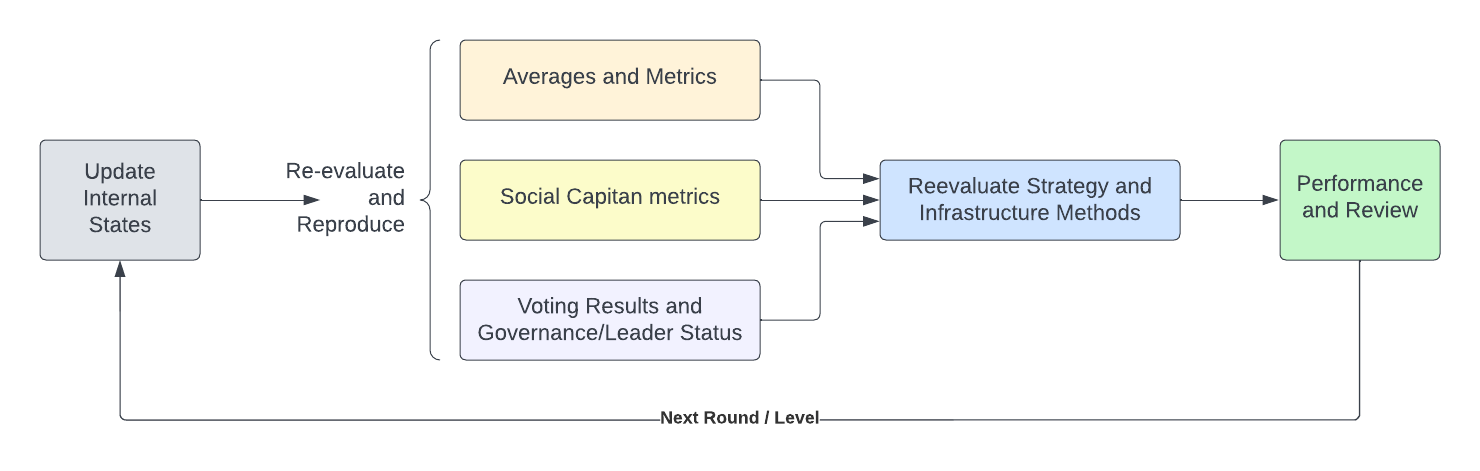
\includegraphics[width=0.8\linewidth]{005_team_2_agent_design/Resources/process.png}
    \caption{Agent Processing per round}
    \label{fig:Process}
\end{figure}

As shown in Figure \ref{fig:Process}, the updated functions described below in the internal state of the agent are run at the end of each level to gather information to be used in the next. These information results and metrics are reevaluated to produce useful data for the strategy and decisions of the agent and are then reviewed through the infrastructure methods implemented. The performance of our agent in terms of its ability to be a good leader is remeasured and stored in one of the agent's metrics to be used in the next rounds to influence our strategy and decisions.

\section{Fighting Decision}
When the agent has to make its own decision, the \verb|FightAction(...)| function is called and returns the decision. Its basic process is illustrated in \autoref{fig:fightaction}.

Each agent contains two character traits, generated at the program's initialisation : \begin{itemize}
    \item \verb|personalTendency| $\in[0,1]$ : the agent's tendency to fight
    \item \verb|replaceTendency| $\in[0,1]$ : the agent's tendency to replace non-fighting agents
\end{itemize}
Additionally, each time \verb|FightAction()| is called, a fluent variable \verb|bravery| is computed such as $$\verb|bravery|(\verb|health|, \verb|stamina|) = \frac{0.5}{1+e^{-0.01(health-500)}} + \frac{0.5}{1+e^{-0.005(stamina-1000)}}$$
which is a combination of two spread logistic functions over the range of \verb|health| and \verb|stamina|.

 \verb|bravery|, $\in [0,1]$, represents the current "confidence"\footnote{The variable bravery was not named confidence in order to avoid mistaking it with the confidence in the leader.} an agent has depending on its state : the more health and stamina it has, the braver it feels.

\begin{figure}[htb]
    \centering
    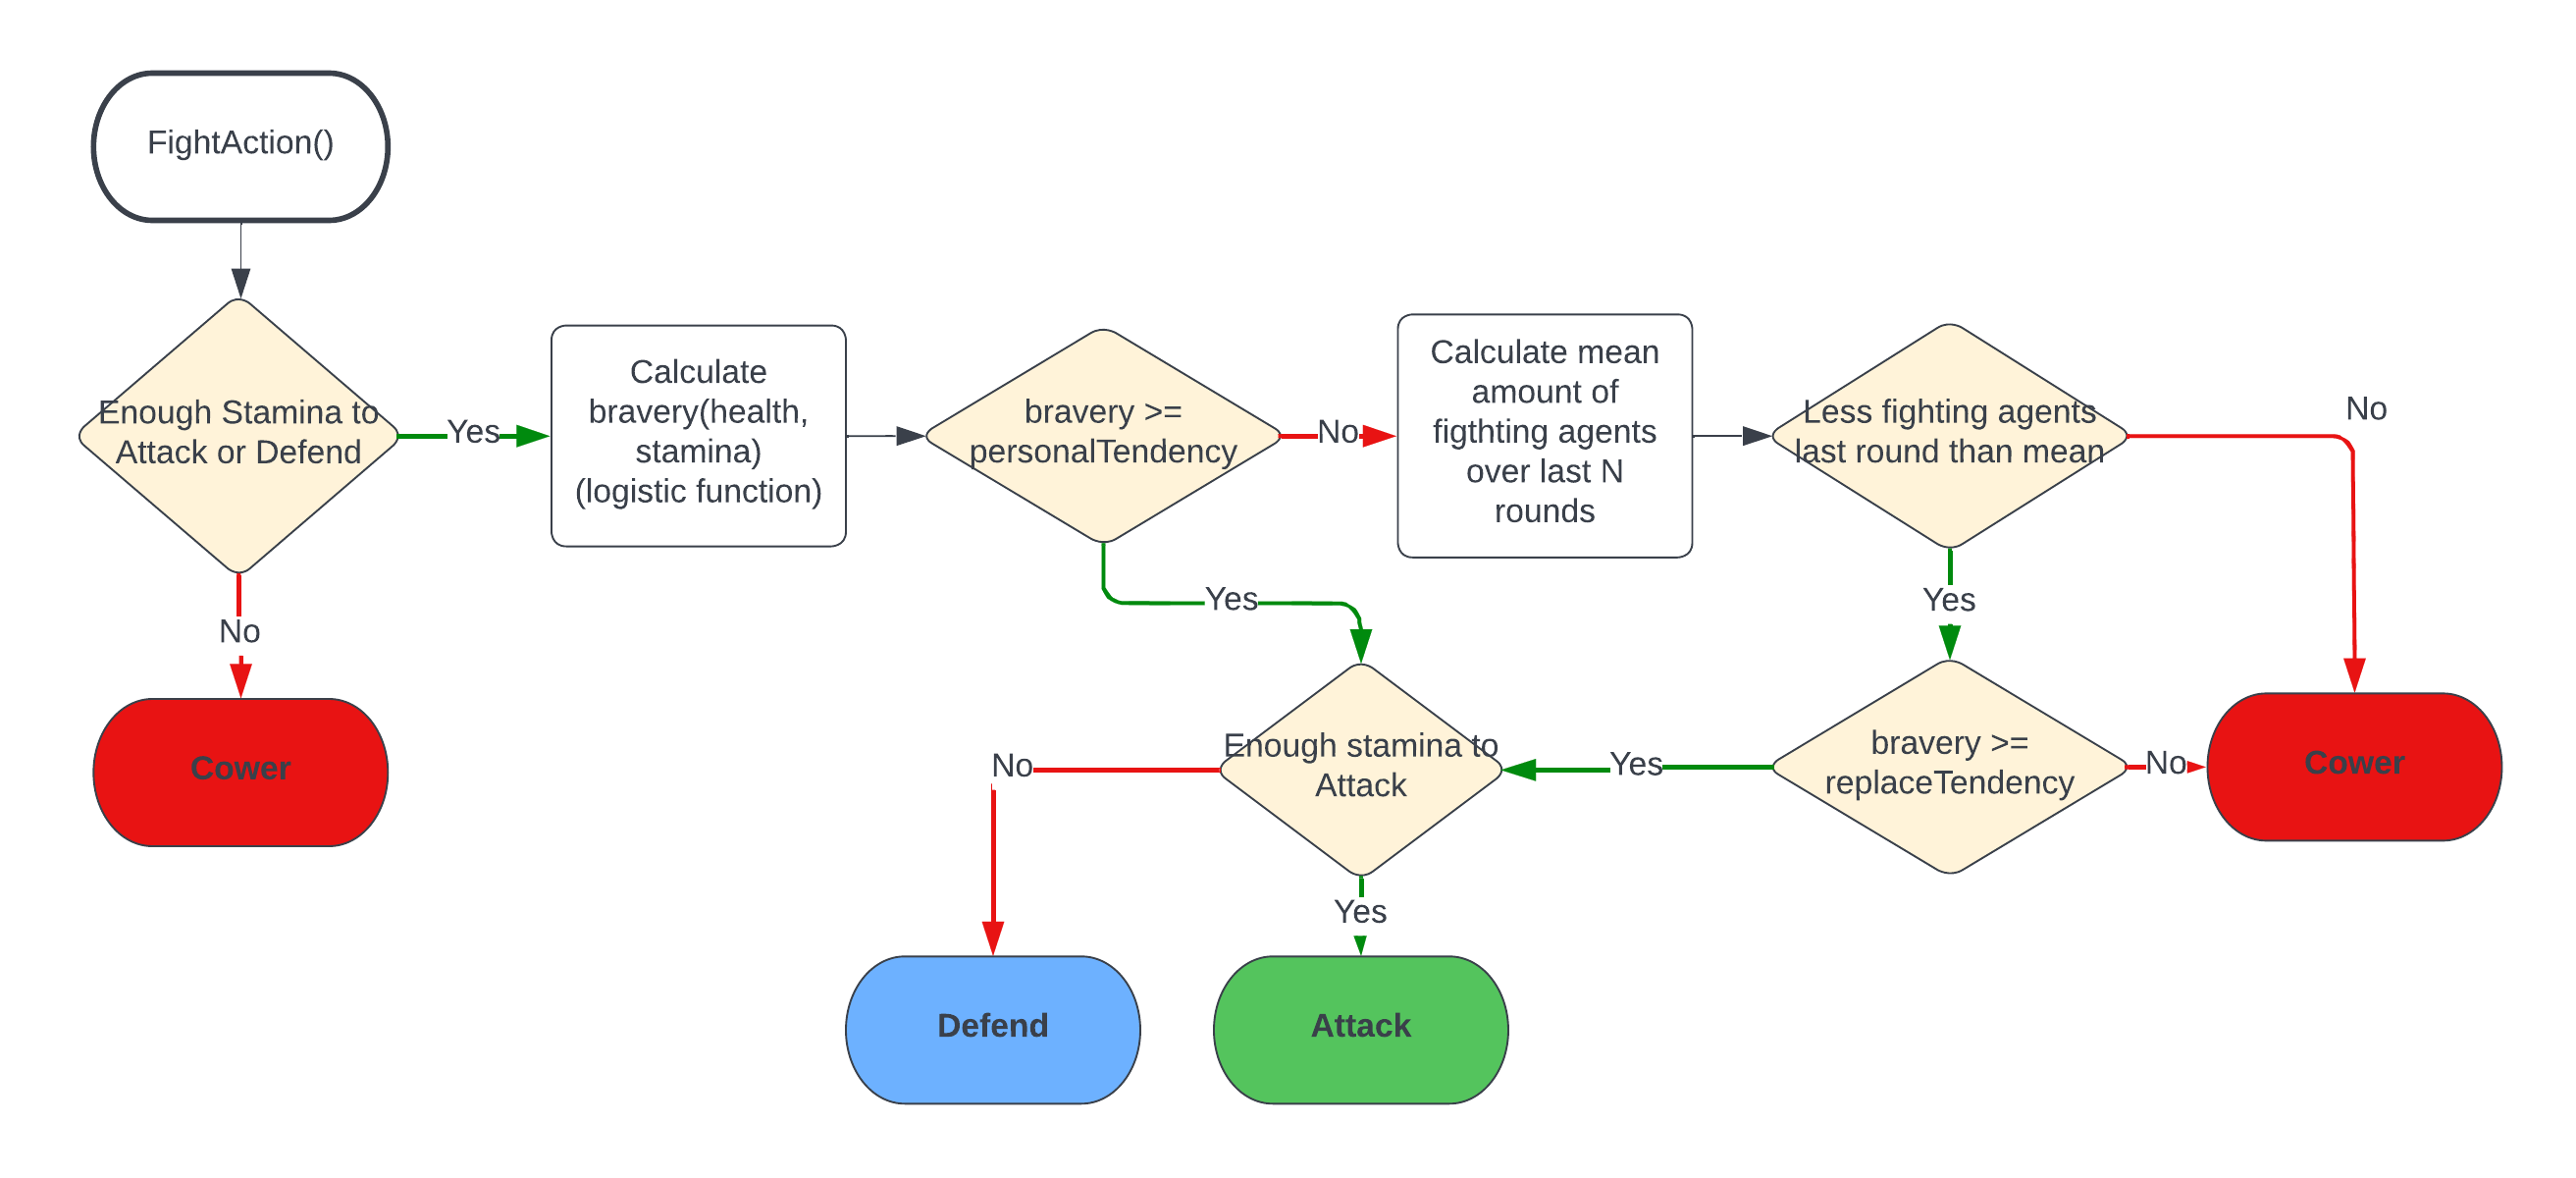
\includegraphics[width=0.8\linewidth]{005_team_2_agent_design/Resources/fightaction.png}
    \caption{Process of personal decision making}
    \label{fig:fightaction}
\end{figure}

 \paragraph{Initial decision}

 By comparing its current \verb|bravery| to its \verb|personalTendency|, the first makes a decision to act or cower. If $\verb|bravery| > \verb|personalTendency|$, it will end the function and return either Attack or Defend. If not, it will first decide to cower.


 \paragraph{Replacement decision}

 If the answer to the initial decision was Cower, the agent will then use the history mechanism (its memory) to observe the overall trend in decisions. It computes the mean of fighting/defending agents over the last $N$ rounds, and if it find that last round was lower than the mean, it will reconsider its decision.

 Then, if  $\verb|bravery| > \verb|replaceTendency|$, it will either Attack or Defend. Else, it will stay in a cowering state.

\section{Fight strategy} If we are elected as a leader, we will have the following fighting strategy: we will propose that agents with Health lower than the bare minimum should Cower, thus forcing those who are the most vulnerable to survive and regenerate health; agents with Health greater than the baseline and attack and defend greater than the minimum required will be suggested to attack and defend as it is their moral obligation to perform these actions and lead the fight; remaining agents that do not fall within these parameters will be free to perform their own Actions. We will choose to broadcast the proposals of other agents with a similar strategy.
\begin{equation}
\begin{aligned}[b]
Elasticity = \frac{NumO\!f\!AgentsAlive}{MinNumO\!f\!Agents}*w_1 + HpPoints*w_2
\end{aligned}
\end{equation}
Elasticity will be used to allow a range for Minimum and Baseline values to be checked with the Proposal if they are satisfied. This is calculated using a combination of the percentage of agents alive, and a weighted value of the Health pool.
% \paragraph{Not-implemented : damage estimation}

% This part was not implemented because at some point, it was decided on the infrastructure side that agents would not have access to the entire set of current agents decisions, and that peer-to-peer communication would be limited.

% An additional test was supposed to be made, where the agent would try to estimate the current damage and defense based on the current set of decision, and possibly decide to act if it found these values to be too low. The decision would have followed the same process as before.

\section{Manifesto}

Influenced by the concept of Relevant Expertise Aggregation - whereby, to be both 'democratic' and 'epistemic', proposals are made by experts but then voted on by the demos - we thought that we could treat leadership candidacy in the game as a matter of how 'expert' an agent is. As far as the manifesto - which is essentially a collection of values that delimit the institutional power our agent wields, if elected (e.g. longer term length and higher percentage required to depose, in the no-confidence vote, both imply greater power) - is concerned, we can actually make a self-estimate of how 'expert' our agent is, as a leader, and then base the manifesto on that. This ensures that we put forth leadership terms commensurate with our actual performance, as a matter of principle, but also by extension that we will be more likely to be voted, considering the other agents may assess our manifesto relative to our performance, themselves, to decide on whether to vote for us. This quantification metric for 'expertise', which can be also thought as an equivalent indicator of credibility in a trust framework, was set as follows:

\begin{equation}
\begin{aligned}[b]
Expertise =& - w_1 * \frac{TimesOverthrown}{TimesElected} + w_2 * ME
\end{aligned}
\end{equation}

\begin{equation}
\begin{aligned}[b]
&ME = \frac{1}{2} * \frac{TimesElected_{FightDecisionPower} + TimesElected_{LootDecisionPower}}{TimesOverthrown^*}\\ &*\text{with any of the two decision powers in our manifesto.}\\
&*\text{ME: Manifesto Effectiveness}
\end{aligned}
\end{equation}

Through \verb|ManifestoEffectiveness| we can measure how well we perform when we request a fight decision or loot decision. It should also be highlighted that expertise does not always increase, but instead it can decrease as well (so it is different to the concept of experience). In order to derive the term length, we map our expertise to a range between 0 and 4 and add it to a default value of 1. In other words, in the very beginning, if we don't have any expertise at all, we request a term length of 1, (which is reasonable due to our lack of expertise), but as we start to gain expertise the term length will dynamically adjust in the range [1,5]. Moving on to fight decision power, we wanted to be able to take into consideration the previous leaders' manifestos and whether they were deposed, since we thought that perhaps the cohort would not trust a new leader with the same manifesto as a previous leader who was deposed. More specifically, we start by checking whether the previous leader had fight decision power and whether he was deposed. If both are true, we take our expertise and subtract from it a small negative bias. Then, if this total value is greater than a threshold, we set \verb|fightDecisionPower| to true in our manifesto. An equivalent logic has been implemented for determining whether \verb|lootDecisionPower| should be true. Finally, for deriving the no-confidence percentage required for our leader to get deposed, we map our expertise to a range of [-10\%, 10\%] and add this value to a default percentage of 51\%, considering that if we do not have any expertise, a simple majority of 51\% would be a reasonable value, but as we start having more expertise, that value should be dynamic and within the range [41\%,61\%], since a more 'expert' leader is more credible and trustworthy, therefore shouldn't be as easy to depose (and vice versa for a less expert leader).

\section{No-confidence vote}
To handle the no-confidence vote for the leader, at the end of each level, we implement a `social capital framework' whereby we take information about various events that have occurred up to that point in the game - which can be classed into reputation events, interactions, and exercises of institutional power - and convert  into them into a numerical value for the respective form of social capital, namely: 
\begin{itemize} 
\item{Trustworthiness}
\item{`Interactiveness' (can also be thought of as how communicative they are, in a network)} \item{Institutional responsibility, when given institutional power}
\end{itemize}

More specifically, `reputation events' in this case would encompass firstly any time that leader was elected leader in the past (i.e. was deemed `trustworthy' by the cohort) - and, secondly, any time during those terms that they were deposed by a vote of no-confidence (i.e. deemed `untrustworthy' by the cohort). Two useful statistics that can be gleaned from historical data, to quantify this, are thus: \textbf{fraction of levels up to now they were elected leader}, and \textbf{fraction of past leadership terms they were deposed}, prematurely to their official term duration. We then subtract the latter statistic from the former to get a value for a social capital indicator we shall call `trustworthiness'. The functions converting the `raw data' of events to these useful statistics can be thought of as `event handlers'. We use private attributes in our agent to track the `raw data' and then, at the end of each level or leadership (depending on the nature of the statistic), we calculate the summative statistics - and append these to a another private attribute which keeps a sequence of leadership terms and the key statistics from its run. We then reset the other attributes (raw data and calculated statistics) to commence tracking again. 

As `interactions' we consider any time a proposal our agent submits to the leader is broadcast to the rest of the cohort. We can quantify how receptive/communicative the leader is with our agent (which we consider valuable, in a network) by calculating the \textbf{average fraction of proposals we submitted to them that they actually broadcast so far, in their current term as well as in past leaderships terms}. These statistics can be directly treated as a social capital indicator: `interactiveness'. 

Exercising institutional power would comprise any action they undertake as leader that cannot be undertaken by the rest of the agents, such as broadcasting a submitted proposal. The net effect of these exercises of power on the common good of the agent collective - i.e. how responsibly they use it - can be measured simply as the \textbf{average survival rate of the agent collective, at the end of any level}, during the current and any past leadership terms of the leader (this can be calculated by keeping track, through the `raw data' private attributes, of the number of agents alive at the beginning and end of a level, and then performing some simple arithmetic). This again be directly treated as a social capital indicator: `institutional responsibility'. 

We would then weight and sum these social capital indicators to produce a final `score' that we will compare to some threshold to make our social decision to vote whether or not we are confident in our current leader (and thus should/shouldn't depose them). However, in order to ensure the magnitudes of the values yielded are meaningful and useful, we actually should first \textbf{normalize the statistics used to yield social capital values, with respect to their global averages}. That is, e.g. : 

\begin{equation}
    avg\_survival\_curr\_term\_norm := (avg\_survival\_curr\_term-avg\_survival)/avg\_survival
\end{equation}

where avg\_survival is the fraction of agents that survive by the end of a level, averaged across all levels so far. This gives an indication of how much better or worse the leader is performing compared to other leaders, and makes the social indicator value more meaningful in social decision making. For any statistic, this value would typically lie in a -1 to 1 range. 

After normalizing the statistics that comprise them, we can then weight the social capital indicators. Unfortunately, we did not manage to implement dynamic adjustment of the weights (which could perhaps be done by looking at e.g. the survival rate patterns under leaders with certain values for the different social capital indicators, and changing to weight more heavily any of them that tend to be higher amongst the better-performing leaders). Instead, we weight them all equally - except the average survival rate under the current leadership, and the average broadcast rate under the current leadership, which we weight twice as much given that the current performance of the leader can be regarded as more important than past performances. 

Finally, we sum these weighted indicators to yield a final confidence score. If this score is above some threshold, we vote positively, and if not, we vote negatively. Being that, post-normalization, the components of this score fall somewhere around -1 to +1, setting this threshold to 0 means we can vote confidence based on whether the leader is, broadly speaking, more valuable in terms of social capital than average (having average values for all the social capital values would yield a score of close to 0).

\section{Election of a leader}To select a preference for the leader, we again take into consideration two of the metrics used in the social capital framework, but also the manifesto of the prospective leaders. More specifically, to vote for a leader, we compute a score for each prospect leader, based on the following parameters. If the leader requires the ability to propose a fight strategy, we add a small negative bias to the score of the prospect leader. This is, because especially if the leader has not been elected before and has no expertise, we prefer that he does not propose a fight. We rather want that this decision comes from all the agents collectively. Equivalently, we add a small negative bias if the leader requires a loot decision power.

\begin{equation}\label{eq:sot}
\begin{aligned}[b]
SOT_i = map : (Overthrow_{i,ranked} + TermLenght_{i, ranked})_{ranked} \rightarrow [0,1]
\end{aligned}
\end{equation}

Additionally, another parameter that we take into account is the sot(overthrow percentage+term length) as seen in equation \ref{eq:sot}. We sum the overthrow percentage and term length for each prospect leader and then rank them in descending order (the one with the smallest overthrow percentage+term length gets the highest points) and normalize them. Now, if the leader has been elected before, we also consider two other parameters used by the social capital metrics produced. These are shown in equations \ref{eq:avgsurv} and \ref{eq:deposed}.

\begin{equation}\label{eq:avgsurv}
\begin{aligned}[b]
AvgSurvivalRateUnderLeader = \frac{\sum_{i} ^{terms} \sum_{j}^{levels} survival\_rate_{i,j}}{\sum_{i}^{terms} \sum_{j}^{levels} 1}
\end{aligned}
\end{equation}

\begin{equation}\label{eq:deposed}
\begin{aligned}[b]
FracTermsDeposed = \frac{NumO\!f\!TimesDeposed}{NumO\!f\!TimesElected}
\end{aligned}
\end{equation}

These parameters are updated per round and outline the average rate at which agents survived per round during the candidate's previous term and the frequency at which the candidate was deposed in his previous terms.
Finally, we weigh these parameters, we sum them and we vote for the agent with the highest score. The highest weights are given to the parameters associated with past leadership data, because we think that expertise is crucial for a leader.\\

\section{Loot Allocation}

\begin{figure}[!ht]
    \centering
    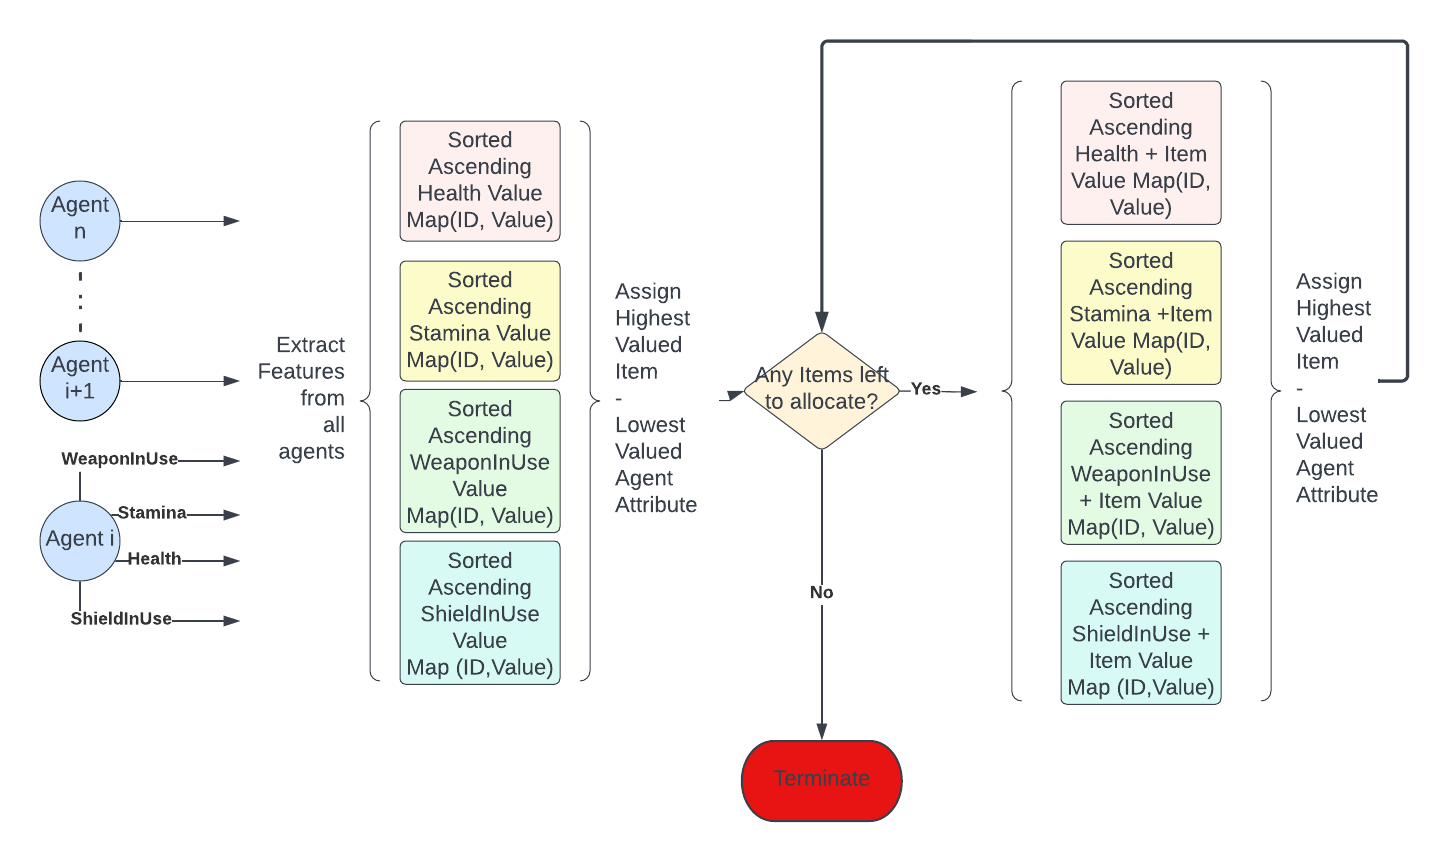
\includegraphics[width=0.8\linewidth]{005_team_2_agent_design/Resources/lootAllocation.png}
    \caption{Loot Allocation Leader Strategy}
    \label{fig:loot}
\end{figure}
The decisions made for the Loot by our agent would be different depending on whether our Agent would be a Leader or not. In the case where our agent was not a Leader at the time of the Loot allocation, our agent would vote on a leader's proposal or on a proposal made by an agent and broadcasted by the leader based on the loot allocated to our agent. If the loot allocated to our agent was found to be different to that of our needs then the proposal would be rejected. If the loot allocated would be similar in type to that of our preference then the proposal would be voted for.
Alternatively, if our agent was elected a leader at the time that would mean that our agent would have to consider apart from its individual interest the greater good of the group. The function of our agent in allocating the loot during leadership can be seen in figure \ref{fig:loot}.

Features regarding the current health, stamina and weapons and shield used by agents are extracted. These are then sorted in arrays for each of the 4 categories to allow the loot to be allocated. Resources are allocated in an egalitarian to secure for everyone an equal set of resources and an equal opportunity to convert those resources into welfare. Consequently, the loot is allocated to in descending value to the ascending sorted arrays of the 4 resource categories of the loot to ensure that all agents have the chance to survive in the following rounds.
Additionally, if there are more resources to be allocated after the first round of allocations the array of the four categories will be re-sorted while taking into account previous rounds' allocations.

\section{Weapon and Shield selection}
Considering that our agent can only attack or defend if our stamina is greater than the damage our weapon or shield can deal respectively, to allow our agent to yield it, as this is a requirement by the infrastructure; we decided that whenever our agent chose to attack or defend, the agent should yield the weapon with the highest damage points lower than our stamina. 
\begin{figure}[!ht]
    \centering
    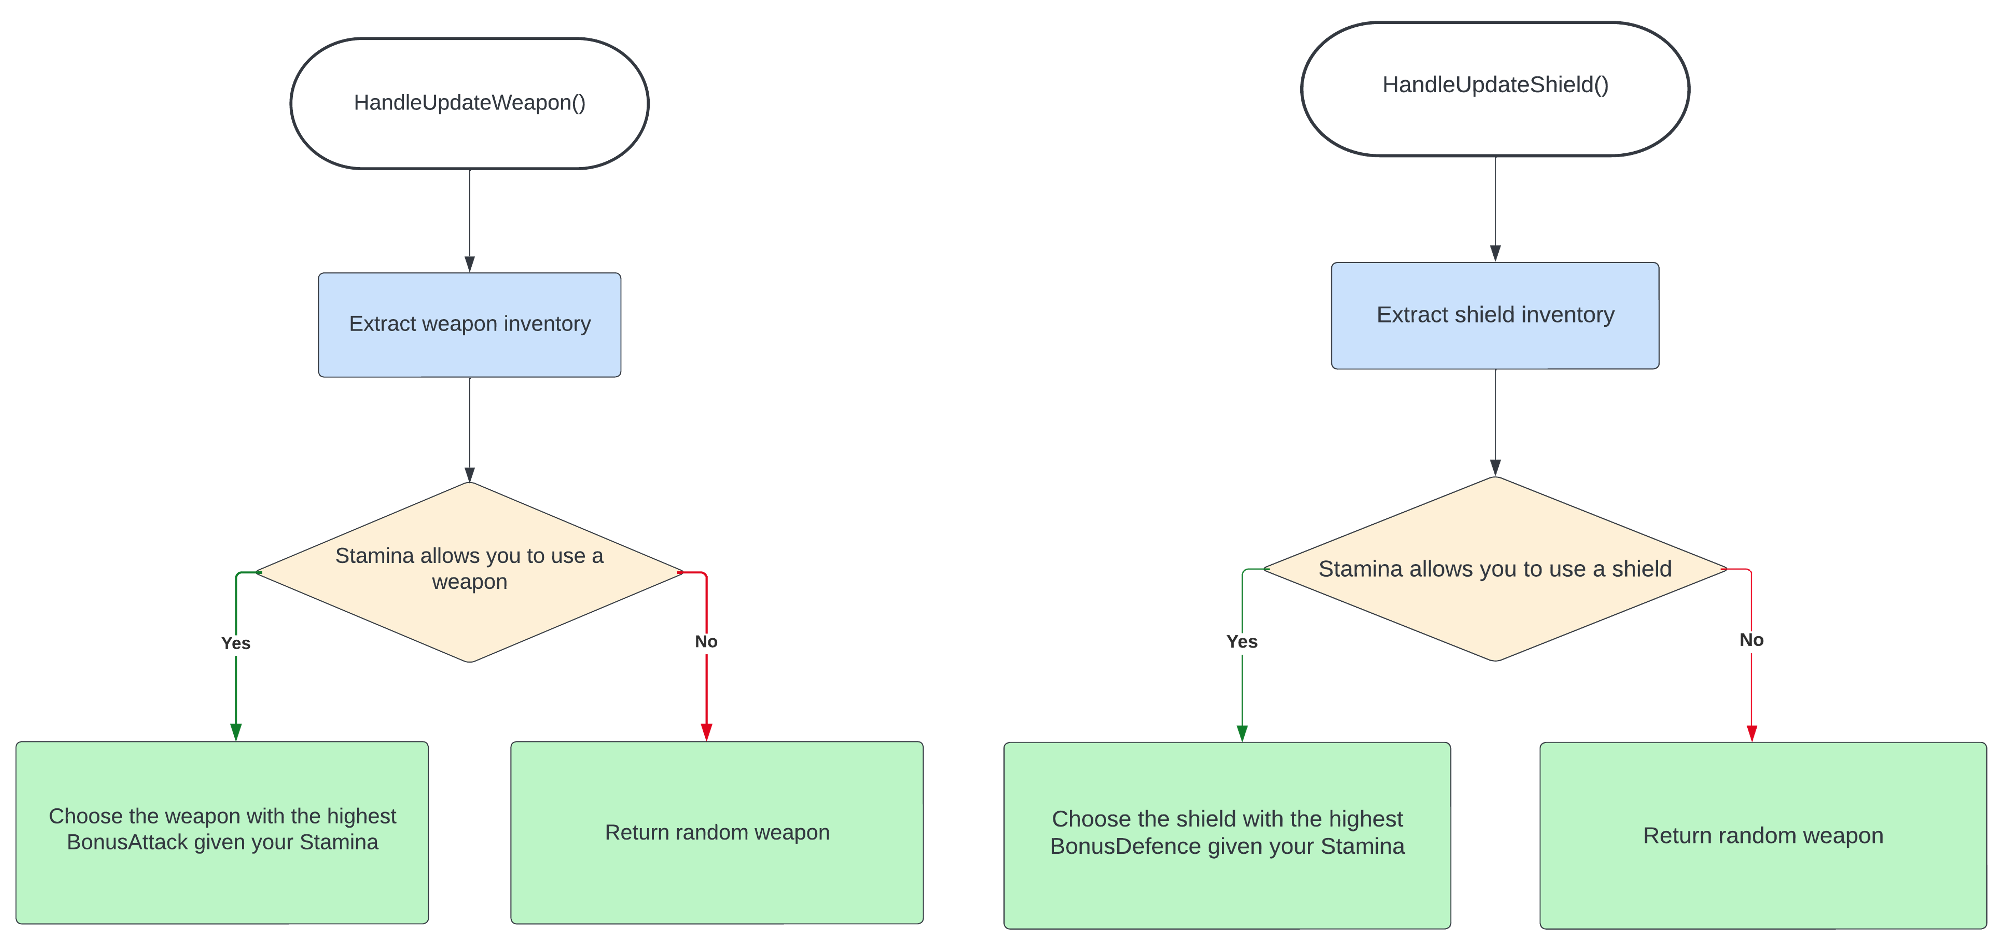
\includegraphics[width=0.6\linewidth]{005_team_2_agent_design/Resources/handleUpdate.png}
    \caption{Weapon and Shield Selections}
    \label{fig:handleUpdate}
\end{figure}

This is outlined in figure \ref{fig:handleUpdate}. This would allow our agent to fight at all times until forced to cower by the infrastructure when our Stamina is fully depleted.

\section{HP pool donation}In terms of HP(Health Points), our agent always donates to the common pool if his health points our greater than a threshold. The amount of health points given at the end of each level is dynamically adjusted according to: 
\begin{equation}
\begin{aligned}[b]
Dynamic \space Donation = H_p * \frac{\Delta H_p}{CurrentLevel}
\end{aligned}
\end{equation}


\section{Agent Performance}
Finally, regarding our agents performance the following metrics have been extracted:
\begin{enumerate}
    \item Reaching level 28 with 58 remaining (with donations to HP pool).
    \item Reaching level 30 with 47 remaining (with donations to HP pool).
\end{enumerate}
These metrics were run with just our agent and with the 60 levels. We believe that based on how our agent has been designed we require the introduction of other agents to allow better performance. This is because our agent always takes into account the greater good and decisions of other agents.